\section{La Nebulosa de Orión}
\section{Estrellas ``Errantes''}
\section{Discos Protoplanetarios}
\section{Proplyds}
\subsection{Descubrimiento}
Observaciones en óptico de la región del trapecio en filtros de banda
angosta de diferentes líneas de emisión tales como $H\alpha$, $H\beta$,
$[OIII]$, $[NII]$, $[SII]$ y continuo, revelaron la existencia de
objetos puntuales únicamente visibles en líneas de alta ionización
($H\alpha$, $H\beta$ y $[OIII]$) que fueron inicialmente denominados como
``condensaciones nebulares'' \citep{Laques:1979}. 

Hasta el momento no se sabía con certeza si ``condensaciones nebulares''
eran en realidad condensaciones nebulares (regiones donde la densidad de
la nebulosa es inusualmente alta por alguna razón o bien esferas de gas
molecular cuya envolvente fue ionizada y que la radiación de la estrella
central la está ``erosionando'') o si se trataba de protoestrellas
de baja masa cuyo disco protoplanetario estaba siendo fotoevaporado por
la estrella central \citep{churchwell:1987}. No fue sino hasta que se contó
con observaciones de alta resolución con el Telescopio Espacial Hubble (HST)
que se se pudo determinar la verdadera naturaleza de estos objetos
\citep{ODell:1993} y la razón por la que se les denominó ``proplyds''
(PROtoPLanetarY DiskS). A su vez se encontraron por primera vez arcos
delgados y otras estructuras de gran interés.

\subsection{¿Qué es un proplyd? Breve introducción \citep{Johnstone:1998}}

Las imágenes del HST de la Nebulosa de Orión mostraron imágenes de discos
alrededor de estrellas jóvenes de baja masa. Algnuos se ven como siluetas
oscuras que contrastan con la nebulosa, y otros casos son visibles en
líneas de emisión de líneas de alta ionización. Un proplyd típico tiene forma
cometaria, con una cabeza brillante que apunta hacia la fuente de radiación
ionizante, y una cola que se extiende en dirección contraria a ésta. La explicación
a esta forma es que el disco protoplanetario está siendo fotoevaporado por la
radiación ionizante de una estrella masiva ($\theta^1~C$ en caso de la Nebulosa
de Orión), la cabeza es un frente de ionización cuyo radio escala como
$R_{IF} \propto D^{2/3}$, donde $D$ es la distancia a la estrella masiva. La forma
de la cola se debe a radiación ionizante difusa, producto de dispersión por polvo
y por recombinaciones (Figura \ref{fig:prop-shape})

\citet{churchwell:1987} ya había notado que la tasa de pérdida de masa observada
en el gas ionizado implicaba que la fuente de este gas debía oscurecer a la
protoestrella huésped, a menos que proviniera de un disco circumestelar. De la
emisión de radio observada, se estima la densidad electrónica en
$n_e \sim 10^6~cm^{-3}$ y la tasa de pérdida de masa en
$\dot{M} \sim 10^{-7}~M_\odot~yr^{-1}$.

\begin{figure}
  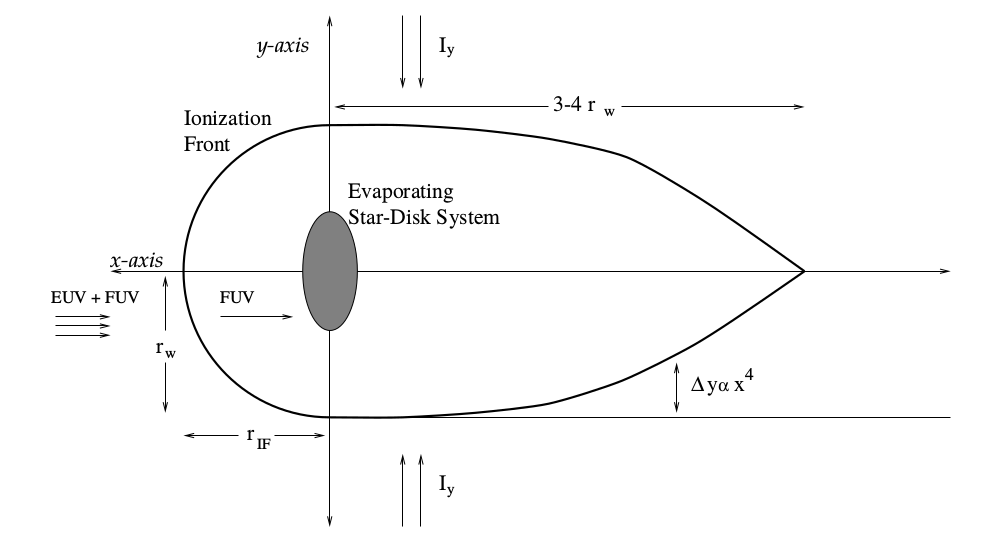
\includegraphics[width=0.8\linewidth]{./Figures/Johnstone-shape}
  \label{fig:prop-shape}
  \caption{Representación esquemáica de la formación de un frente de ionización
    hemisférico y de una cola de gas ionizado detrás del disco en proceso de
    fotoevaporación. $r_{IF}$ y $r_w$ representan el radio del frente de ionización
    en las direcciones de los ejes $x$ e $y$, respectivamente. $I_y$ representa el
    campo de radiación difusa. Por detrás del disco, la radiación difusa calienta el
    gas del disco provocando otro flujo fotoevaporado. $\Delta y$ es la diferencia
    entre la forma actual del frente de ionización por detrás del disco y una forma
    cilíndrica. La forma de la colase explica como que el flujo de radiación $I_y$
    es capaz de penetrar más cerca del eje $x$ conforme uno se aleja del disco, donde
    el flujo fotoevaporado es menos denso.}
\end{figure}


\subsection{Mecanismos de fotoevaporación \citep{Johnstone:1998}}

El principal mecanismo de fotoevaporación es el campo de radiación de la
estrella central, especialmente en la parte ultravioleta del espectro
electromagnético. Según la masa de la estrella central, podemos tener dos
clases de flujo radiativo: Dominado por el ultravioleta lejano (FUV,
$h\nu < 13.6~eV$) o dominado por el ultravioleta extremo (EUV,
$h\nu \geq 13.6~eV$). En general, el FUV se encarga de disociar moléculas
y de calentar el gas de la región de fotodisociación (PDR) hasta
temperaturas de 100 - 1000 K, mientras que el EUV puede ionizar el gas y
elevar su temperatura hasta $10^4~K$. El EUV no puede atravesar el frente
de ionización (IF) pero el FUV sí.

En el caso de que el flujo sea dominado por el EUV, la presión térmica del
flujo fotoevaporado es determinada por la fotoionización, la PDR producida
por el FUV es delgada. El gas calentado por el FUV se mueve de manera
subsónica hasta llegar al IF y la tasa de pérdida de masa
depende de la tasa de ionización inducida por el EUV.

Si el flujo está dominado por el FUV, la presión térmica depende del
calentamiento por el FUV. El gas tibio se expande como un viento que empuja
el IF lejos del disco. La tasa de pérdida de masa la determina la temperatura
de la PDR, el flujo FUV y la opacidad del polvo a las longitudes de onda del FUV.

Inicialmente la forma del disco impone una geometría cilíndrica en el
flujo fotoevaporado, pero eventualmente los gradiente de presión tornan
esta geometría en esférica.

Las ecuaciones de continuidad de la masa y el momento restringen la velocidad
del flujo neutro antes de alcanzar el IF. Mas allá de éste, la presión del
gas hace que éste se expanda a velocidades del orden de una a dos veces la
velocidad del sonido. Para el gas neutro dentro del IF hay dos posibles
soluciones: si el gas neutro es supersónico entonces el IF será de baja
densidad (Tipo R) con bajo contraste de densidad entre gas neutro y
gas ionizado. O si el gas neutro es subsónico se formará un IF tipo D con un
gran contraste de densidad entre el gas neutro y el gas ionizado. Sin embargo,
sin importar qué tipo de radiación domina la fotoevaporación, el gas neutro
permanece a velocidades subsónicas al llegar al IF, por lo que dicho frente
será tipo D. 
En el caso de un flujo dominado por el EUV, el gas neutro permanece a
velocidad subsónica, su velocidad decae como $v_I \propto r^{-2}$ y llega
a $0.5~kms^{-1}$ al llegar al frente de ionización. Cundo el flujo es
dominado por el FUV, el gas neutro se acelera hasta llegar a velocidades
supersónicas, luego atraviesa un choque isotérmico que lo desacelera y
llega al frente de ionizacion a $0.5~kms^{-1]$.

  \begin{figure}
    \begin{tabular}{cc}
      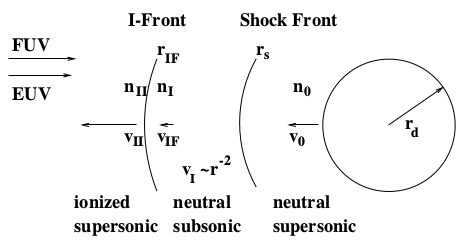
\includegraphics[width=0.5\linewidth]{./Figures/Johnstone-2} &
      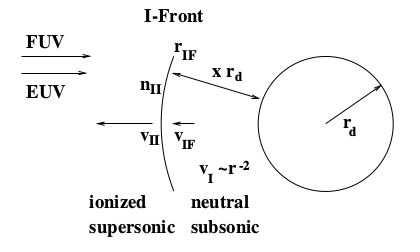
\includegraphics[width=0.5\linewidth]{./Figures/Johnstone-3}
    \end{tabular}
    \label{fig:EUV-FUV-IF}
    \caption{Representación esquemática de las regiones del flujo
      fotoevaporado de un proplyd. Izquierda: Cuando el flujo es dominado
    por el FUV. Derecha: Flujo dominado por EUV \citep{Johnstone:1998}}
  \end{figure}
  

Sin importar el tipo de mecanismo de fotoevaporación dominante, el flujo
fotoevaporado solo si la presión térmica supera a la gravedad de la
protoestrella. Entonces, el flujo fotoevaporado solo existe a partir de
un radio crítico $r_g$, donde este radio se estima a partir del balance
entre la energía necesaria para escapar de una órbita kepleriana y la
energía térmica:
\begin{align}
  r_g = \frac{GM_*}{a^2}
\end{align}
Donde $M_*$ es la masa de la protoestrella y $a$ es la velocidad del sonido
del gas. Para las protoestrellas típicas del trapecio la masa típica es de
$M_* = 0.2~M_\odot$. Para el gas neutro la velocidad del sonido es de
$a_I \sim 3~km~s^{-1}$ y para el gas ionizado es de $a_{II} \sim 10~km~s^{-1}$.
Por tanto, el radio gravitacional para un flujo dominado por el EUV es de
$r_{gII} \sim 2~AU$ y para un flujo dominado por el FUV es de
$r_{gI} \sim 20~AU$.
\section{Objetos LL}
\subsection{Mapa de Objetos}